%!TEX root = batch-course.tex
%-------------------------------------------------
\section{Batch analysis via direct PCA and PLS}
%-------------------------------------------------

\begin{frame}\frametitle{Batch systems: simple definition}

\begin{exampleblock}{Simplest definition}
\centering{\large{\textbf{A batch system}: group of the \alert{\emph{same variables}}, gathered over a period of \alert{\emph{time}}}}
\end{exampleblock}
	
\begin{center}
	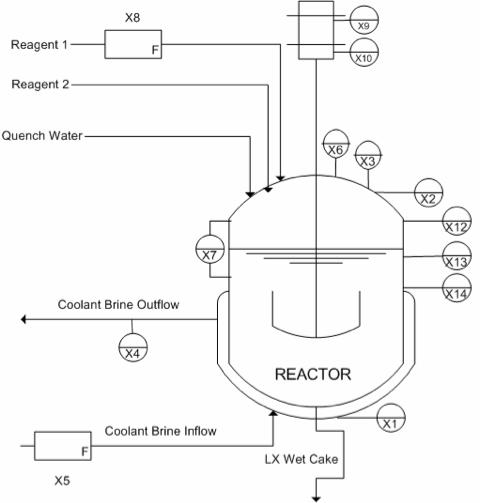
\includegraphics[width=6cm]{images/batch-system.png}	
\end{center}

\end{frame}	

\begin{frame}\frametitle{Batch systems: changing relationship}

	\textbf{Batch system}: group of the \emph{same variables}, gathered over a period of \emph{time}.  Why not just use ordinary PCA or PLS:

	\begin{center}
		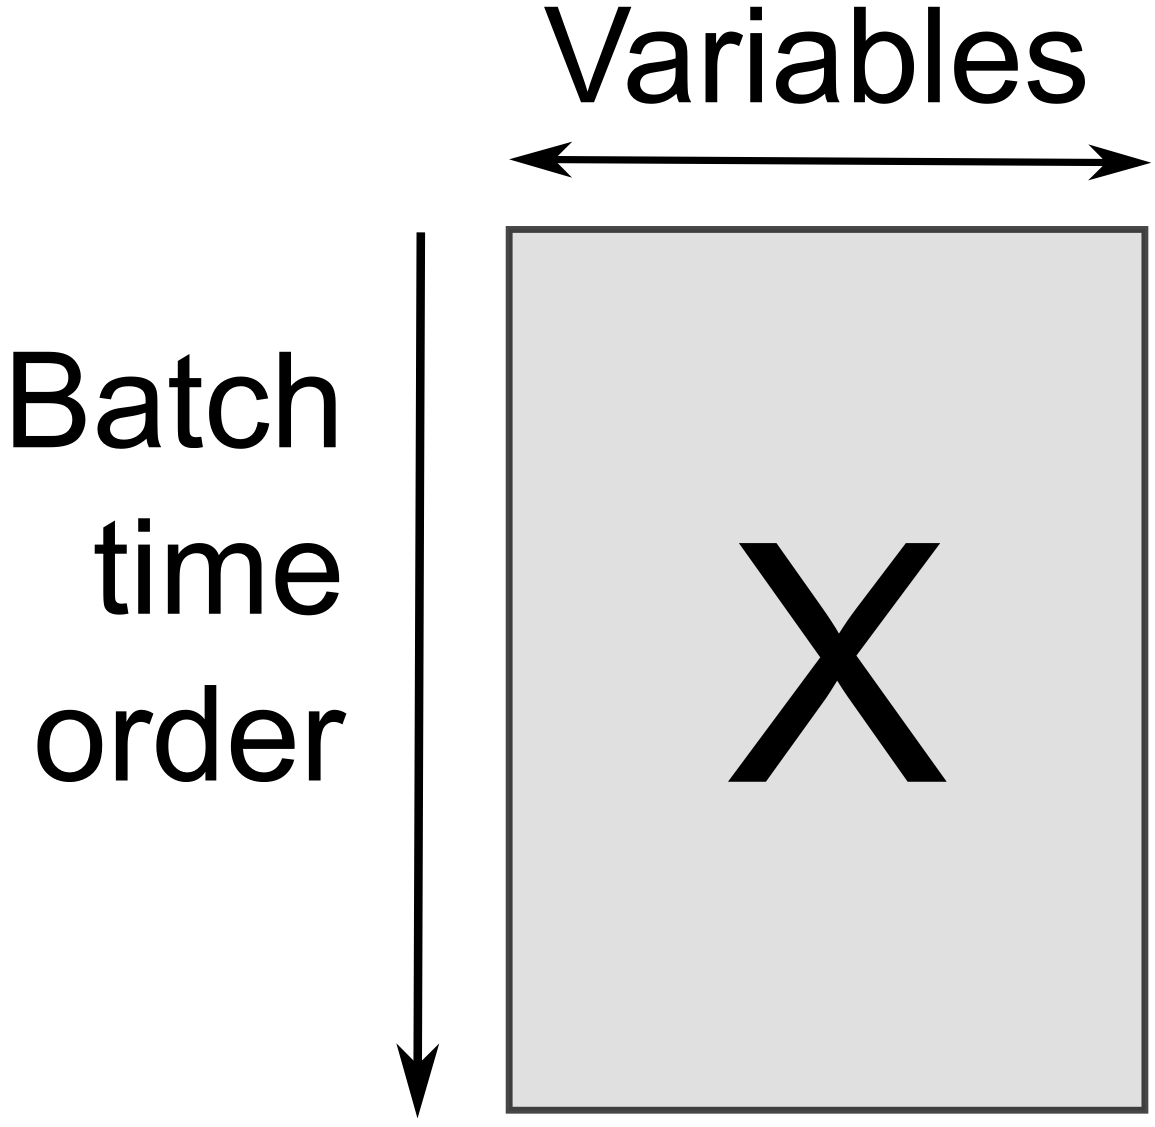
\includegraphics[width=2.0cm]{images/batch-illustrate-unusual-unfolding.png}
	\end{center}

	\begin{itemize}
		\item 	PCA is invariant to row order: 
		\begin{itemize}			
			\item	can shuffle rows, still get same model
			\item 	PCA explains how rows are related to each other
			\item 	each row is assumed independent of the others
			\item 	summarizes relationship between variables (columns)
		\end{itemize}
	\end{itemize}

	\begin{exampleblock}{Key issue}
	In \textbf{batch systems}: relationship between variables \alert{changes during the batch}.  So the above approach is not appropriate.
	\end{exampleblock}
\end{frame}

\begin{frame}\frametitle{Batch systems: changing relationship}

\begin{enumerate}
	\item Relationship between variables change within a batch 
			\begin{itemize}
				\item 	Entry and exit temperatures in a batch dryer correlate (move together) at the end of the batch. 
				\item 	But, at start of the batch there is little relationship: heat used to evaporate moisture	
			\end{itemize}

	\pause
	
	\item Past history of a batch affects future behaviour: a batch is an ``integrating system''
	
			\begin{itemize}
				\item 	Unfolding batch data as shown previously won't capture that ``past effect'' on future rows.  Why?
				
				\pause
				
				\item  	Recall: each row is independent in PCA and PLS
			\end{itemize}

\end{enumerate}
\end{frame}

\begin{frame}\frametitle{Batch systems: changing relationship}
\begin{enumerate}
	\setcounter{enumi}{2}
	\item 	Predictive modelling is harder by unfolding this way

			\begin{center}
				\includegraphics[width=3.5cm]{images/batch-illustrate-unusual-unfolding-with-Y.png}
			\end{center}
			
		
			\begin{itemize}
				\item 	What do we use as the \( \mathbf{Y} \) matrix in this case? {\scriptsize We don't have  \( \mathbf{Y} \) values at each time step.}
				\item 	Many elaborate schemes proposed in literature.			
			\end{itemize}
		
	\item 	Simple solution: arrange data so that each batch is within a row
	
			\begin{itemize}
				\item 	There are some issues with this  (alignment, real-time monitoring)
				\item 	In general, these issues can be addressed effectively
			\end{itemize}
\end{enumerate}
\end{frame}

\begin{frame}\frametitle{Analysis and learning from batch data}

	\begin{exampleblock}{Approach}
	Unfold the aligned batch data row wise, one batch per row, and use PCA and PLS directly.
	\end{exampleblock}

	\begin{center}
		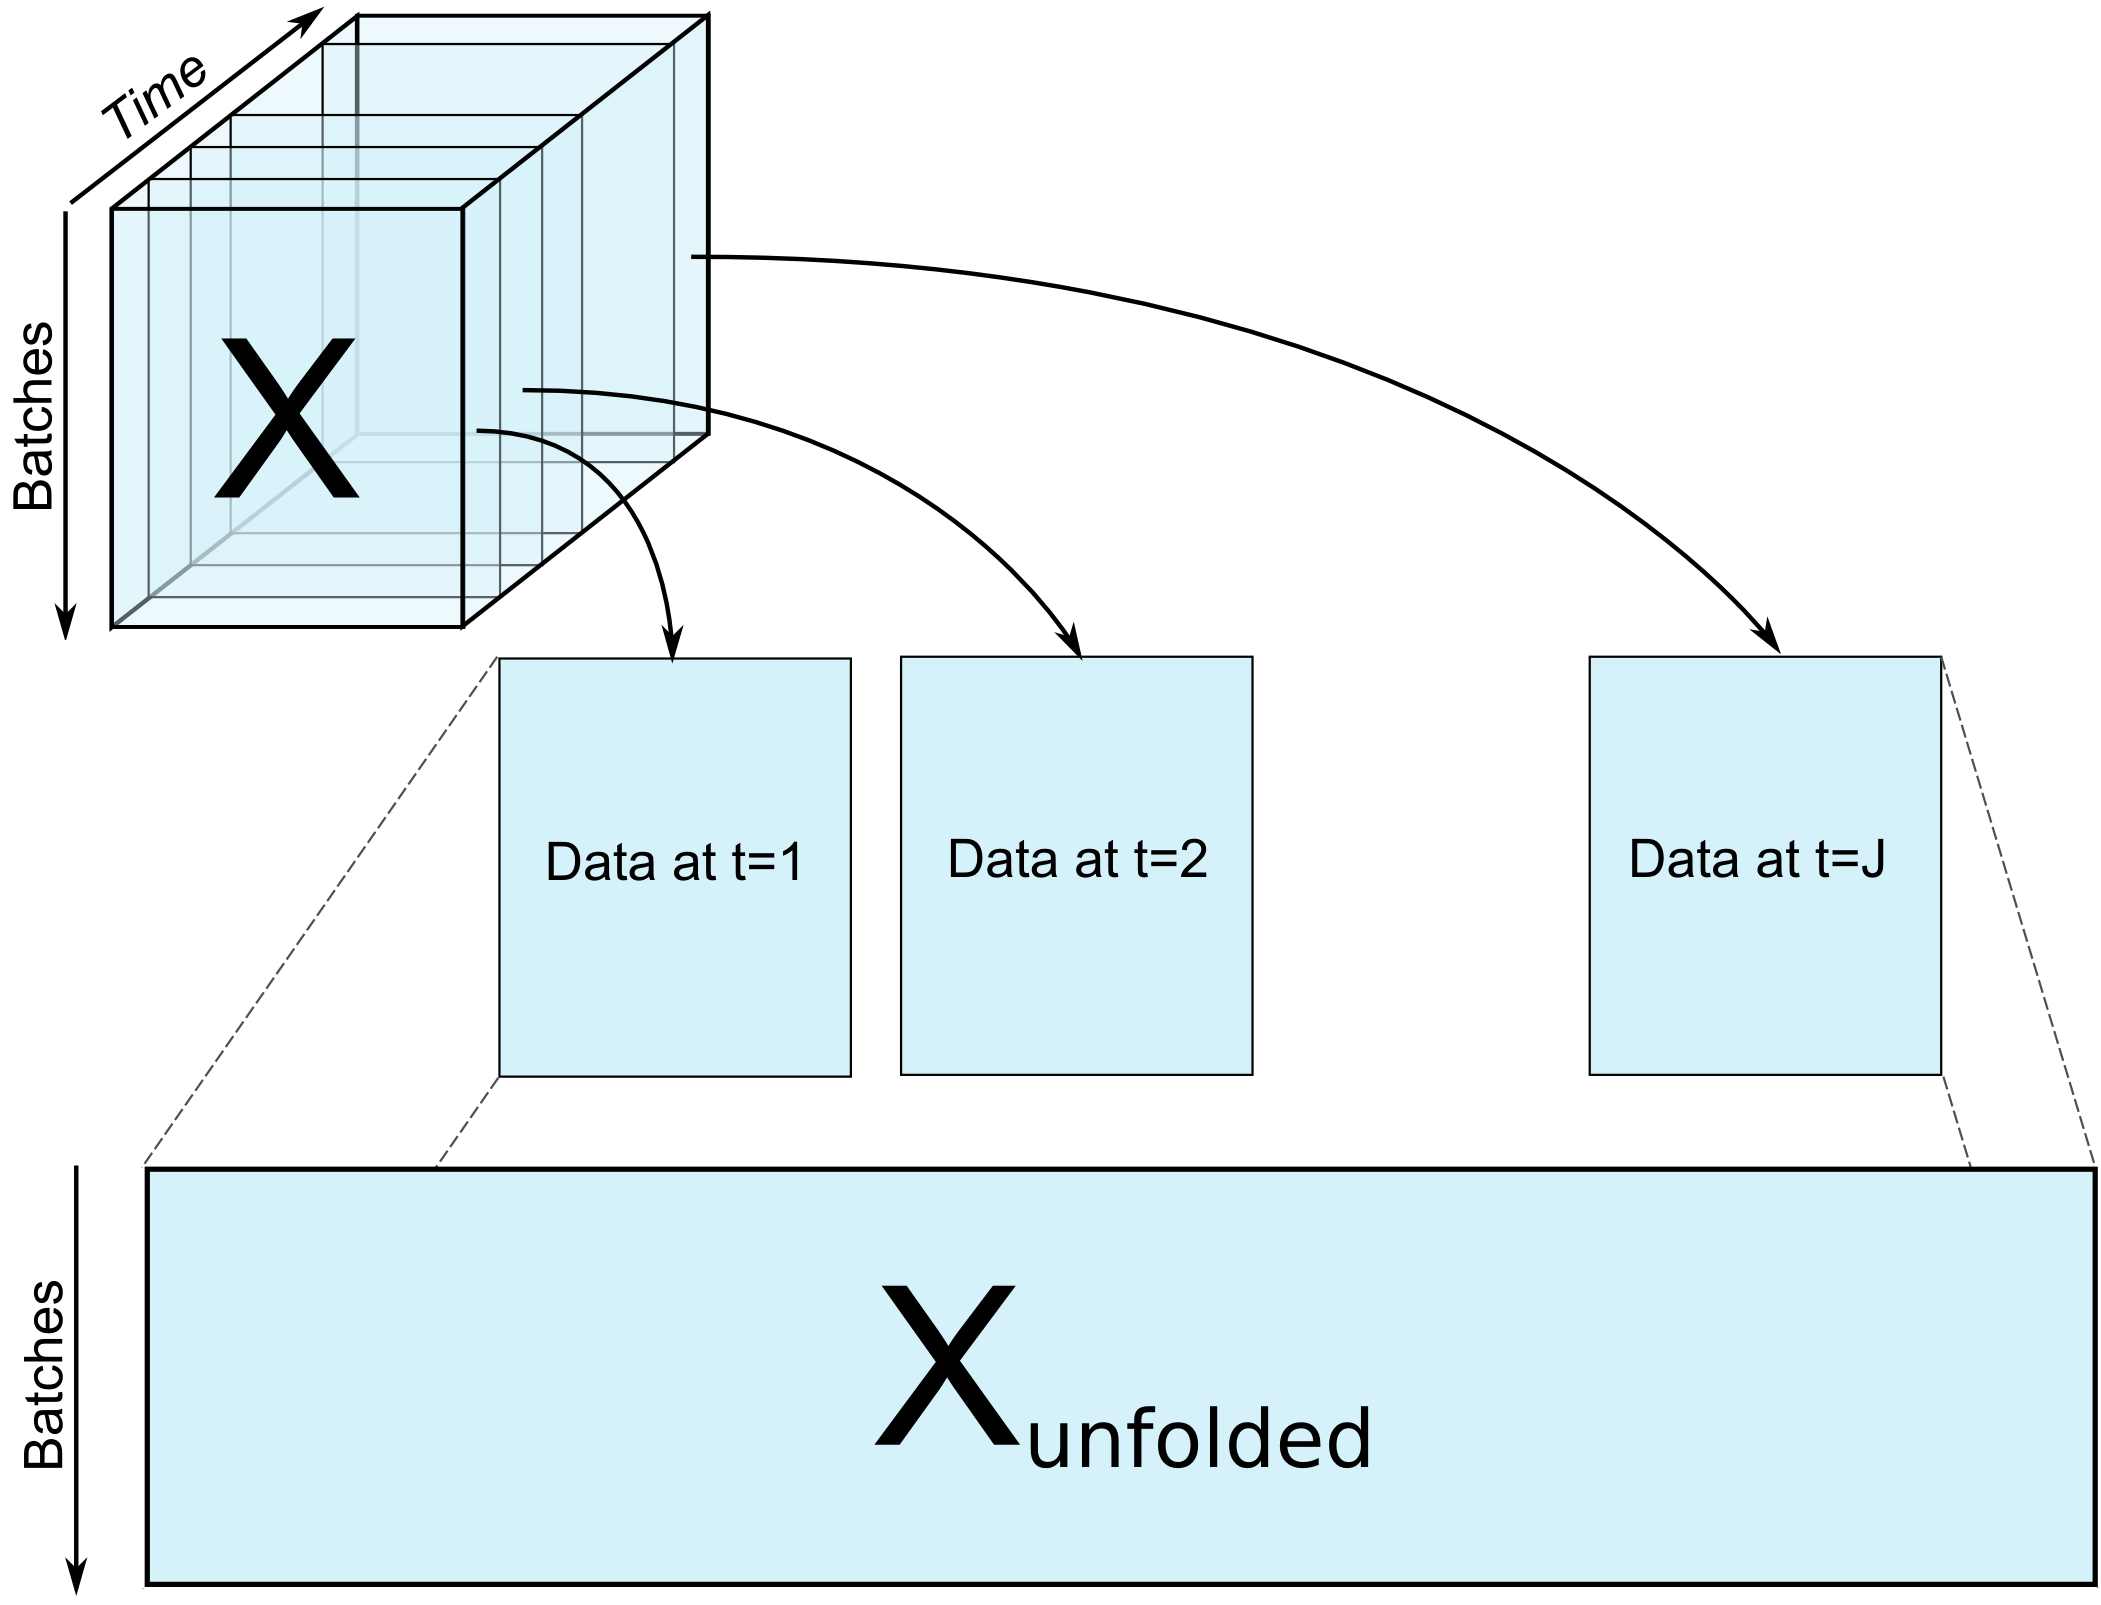
\includegraphics[width=8cm]{images/batch-data-unfolding-X-only.png}	
	\end{center}
\end{frame}	

